\section{Introduction}

The optimisation of fermentation processes involving filamentous microorganisms requires an in-depth knowledge of the relationship between biomass and metabolite production. The specific morphological form adopted by an organism, which is dependent on a variety of factors \cite{znidarsic2001}, is of critical importance to the clarification of this dependency, as particular phenotypes are associated with maximum productivity. In particular, the extent to which an organism forms branches is often of interest, as evidence in the literature suggests that metabolite excretion occurs primarily at hyphal tips \cite{gordon2000,muller2002}. With the advent of image analysis systems, significant progress has been made in furthering the understanding of the link between morphology and productivity \cite{papagianni2004}. However, the accurate quantification of complex morphologies still represents a major challenge in process optimisation.

At the macroscopic level, the dispersed mycelial morphological form may dominate, or an aggregation of \lq free' hyphal elements may result in mycelial \lq clumps' being predominant. Alternatively, dense pellet structures, which may be up to several millimetres in diameter, may result from the aggregation of spores prior to germination, the aggregation of spores and germ tubes or the aggregation of mycelia. In fermentations of certain microorganisms, such as \emph{Aspergillus oryzae} and \emph{Aspergillus terreus}, there is evidence that pellet-formation is driven by spore agglomeration \cite{carlsen1996a,bizukojc2009} and, as such, the occurrence of \lq free' mycelia may be rare. The characterisation of these complex macro-morphologies represents a far greater challenge to the fungal biotechnologist, as individual hyphae cannot be isolated and enumerated. As such, the accurate determination of the extent of branching of the organism is often impossible. These large aggregates of biomass are conventionally characterised in terms of projected area ($\Ap$), perimeter length ($P$), circularity ($C=4 \pi A_p P^{-2}$), or various other interpretations thereof \cite{papagianni2006a,tucker1992,li2002}. As different morphological parameters are often utilised depending on the growth form present, a considerable amount of effort has been expended in designing imaging systems capable of discriminating between these different phenotypes \cite{papagianni2006a,tucker1992}. An alternative approach to morphological quantification employs the use of fractal geometry to characterise the spatial distribution of an organism.

\subsection{What are fractals?}

The term \lq fractal' geometry, derived from the Latin \emph{fractus} meaning \lq broken' or \lq fractured', was first used by Mandelbrot \cite{mandelbrot1982} to describe objects that are \lq self-similar' (similar at different scales). More specifically, Mandelbrot described a fractal as \lq \emph{a rough or fragmented geometric shape that can be split into parts, each of which is (at least approximately) a reduced-size copy of the whole.}' There are many examples of such objects in nature, such as clouds, mountain ranges, coastlines and snow-flakes. One of the more commonly cited examples of a naturally-occurring fractal is perhaps the fern (Fig.~\ref{fig:FractalFern}), which displays a similar morphology at different scales: a central \lq stem' from which pointed \lq leaves' emerge. Fractal geometry has also been made use of in art (Fig.~\ref{fig:FractalArt}), long before the concept was formalised mathematically.

\begin{figure}[bt]
	\centering
	\captionsetup[subfloat]{labelformat=empty}
	\subfloat{\fbox{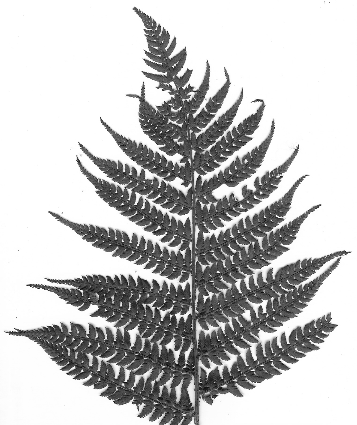
\includegraphics[height=6cm]{../C6/ferna}}}
	\hspace{0.3cm}
	\subfloat{\fbox{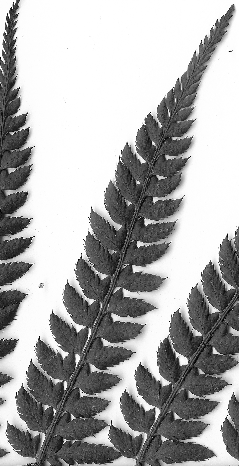
\includegraphics[height=6cm]{../C6/fernb}}}
	\hspace{0.3cm}
	\subfloat{\fbox{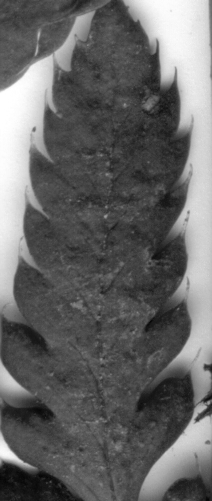
\includegraphics[height=6cm]{../C6/fernc}}}
	\caption{A fern is an example of a naturally-occurring fractal, exhibiting a similar form at different scales.}
	\label{fig:FractalFern}
\end{figure}

\begin{figure}[bt]
	\centering
	\captionsetup[subfloat]{labelformat=empty}
	\subfloat{\label{fig:PersianFractal}\fbox{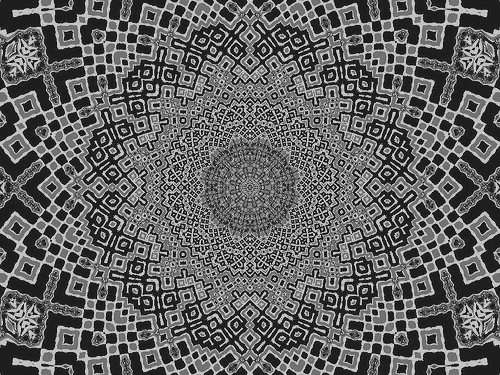
\includegraphics[height=4.5cm]{../C6/PersianFractal}}}
	\hspace{0.5cm}
	\subfloat{\label{fig:hokusai}\fbox{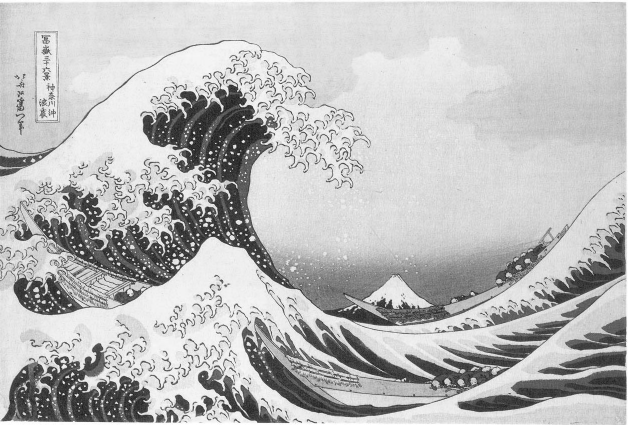
\includegraphics[height=4.5cm]{../C6/hokusai}}}
	\caption{Many examples of Islamic art exhibit fractal properties (left), while self-similarity is clearly visible in Hokusai's \emph{The Great Wave off Kanagawa} (right).}
	\label{fig:FractalArt}
\end{figure}

Several studies have also demonstrated that certain filamentous microorganisms can be considered self-similar structures \cite{papagianni2006b,cpark2007,jones1997,jckim2005,ryoo1999,hitchcock1996,golinski2008}, as do several bacterial strains of Gram-negative rods, under certain conditions \cite{matsuyama1992}. Effects of different grazing densities of collembolans on colonies of the fungus \emph{Hypholoma fasciculare} \cite{kampichler2004} and trophic responses of \emph{Phanerochaete velutina} mycelial systems to nutrient stimuli \cite{wells1998} were also quantified in the same manner. Fractal geometry has also been used as a means of standardising mycelial inocula for submerged fermentations \cite{jones1993a}.

The concept of fractal or fractional dimension may be considered as follows \cite{mandelbrot1967}. Consider a straight line of dimension one and of length $X$. For any positive integer $N$, the segment may be exactly decomposed into $N$ non-overlapping segments of length $X/N$. Each sub-segment may then be considered a scaled version of the original, where $r(N) = 1/N$ is the scaling ratio. This concept may be extended to two dimensions, whereby a rectangle of length $X$ and breadth $Y$ may be sub-divided into $N$ smaller rectangles, each of length $X/\sqrt{N}$ and breadth $Y/\sqrt{N}$, in which case the scaling ratio is $r(N) = 1/\sqrt{N}$. This relationship may be generalised as follows:

\begin{equation}
	r(N) = \frac{1}{N^{1/D}}
\end{equation}

\noindent The fractal dimension ($D$) is therefore given by:

\begin{equation}
	D = -\frac{\log N}{\log r(N)}
\end{equation}

\noindent This principle is illustrated by the construction of the von Koch curves (Fig.~\ref{fig:KochCurve}). Beginning with a straight line of length $X$, the line is divided into three segments, each of length $X/3$. A fourth segment of length $X/3$ is added and the four segments are arranged as shown, producing the triadic von Koch curve. In this case, $r(N)=1/3$, as each of the individual segments is one third the length of the original, and $N=4$. Therefore:

$$D = - \frac{\log 4}{\log 1/3} = \frac{\log 4}{\log 3} \approx 1.262$$

\noindent Alternatively, if $r(N)=1/4$ and $N=8$, the result is the quadratic von Koch curve, for which $D = 1.5$. Iteratively repeating this \lq divide and construct' procedure results in curves of increasing visual complexity, which are not easily described using Euclidean measures. However, the basis for their construction is relatively simple, as is their subsequent decomposition into elementary, geometrically identical sub-structures, and a single dimension ($D$) may be used to describe the curves.

\begin{figure}[htbp]
	\centering
	\captionsetup[subfloat]{labelformat=empty}
	\subfloat[$i=0$]{\includegraphics[width=5cm]{../C6/Kochn0}}
	\\
	\subfloat[$i=1$]{
		\begin{tabular}{m{5cm} c m{5cm}}
			\includegraphics[width=5cm]{../C6/Kochn1} & \hspace{0.5cm} &
			\includegraphics[width=5cm]{../C6/qKochn1}
		\end{tabular}
	} \\
	\subfloat[$i=2$]{
		\begin{tabular}{m{5cm} c m{5cm}}
			\includegraphics[width=5cm]{../C6/Kochn2} & \hspace{0.5cm} &
			\includegraphics[width=5cm]{../C6/qKochn2}
		\end{tabular}
	} \\
	\subfloat[$i=3$]{
		\begin{tabular}{m{5cm} c m{5cm}}
			\includegraphics[width=5cm]{../C6/Kochn3} & \hspace{0.5cm} &
			\includegraphics[width=5cm]{../C6/qKochn3}
		\end{tabular}
	} \\
	\subfloat[$i=4$]{
		\begin{tabular}{m{5cm} c m{5cm}}
			\includegraphics[width=5cm]{../C6/Kochn4} & \hspace{0.5cm} &
			\includegraphics[width=5cm]{../C6/qKochn4}
		\end{tabular}
	} \\
	\caption{The triadic (left) and quadratic (right) von Koch curves, where $i$ denotes the number of iterations.}
	\label{fig:KochCurve}
\end{figure}

\subsection{Quantifying the fractal dimension}

One of the earlier approaches to fractal dimension evaluation, termed the \lq Richardson walk' \cite{richardson1961}, originally described the effect of scale when measuring a coastal perimeter on a map using dividers. As the step size ($s$) is reduced, the measured perimeter ($P$) increases, with more of the coastal irregularities included in the measure. A plot of $\log P(s)$ versus $\log n$ will result in a straight line, the slope of which is related to the fractal dimension ($D$) by:

\begin{equation}
	P(s) = a s^{1-D}
\end{equation}

\noindent where $a$ is a constant. The range of scales over which the expression holds true is obviously limited at the lower end by the resolution of the map and at the upper end by the size of the coastline being measured.

A more accurate implementation of such a method for the analysis of objects in digital images is based on the calculation of a Euclidean distance map (EDM) \cite{russ2002}. The grey-level histogram ($h(x)$) provides the luminance value at each distance ($d$) from the \lq ultimate point', the centre of the EDM. The perimeter, $P$, at a distance $d$ from the object's centre may be calculated according to:

\begin{equation}\label{eq:P(d)}
	P(d) = \frac{1}{d}{\displaystyle \sum_{x=0}^d h(x)}
\end{equation}

\noindent In this instance, $d$ may be thought of as the scale or step size, as a lower value will effectively result in a lower \lq resolution' measure of the object perimeter and vice-versa.  A plot of $ \log P(d)$ versus $ \log d$ produces a straight line (Fig.~\ref{fig:EDMFrac}). However, such an approach is not suitable for the analysis of hyphae, as the EDM of such images typically contains a very small number of grey levels due to the elongated nature of hyphae.

\begin{figure}[htbp]
	\centering
	\subfloat[]{\label{fig:EDMFraca}\fbox{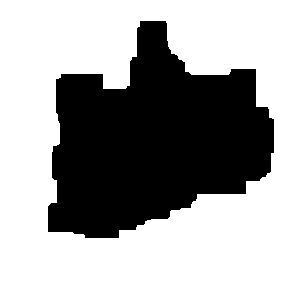
\includegraphics[width=4.5cm]{../C6/EDMFrac}}}
	\hspace{0.5cm}
	\subfloat[]{\label{fig:EDMFracb}\fbox{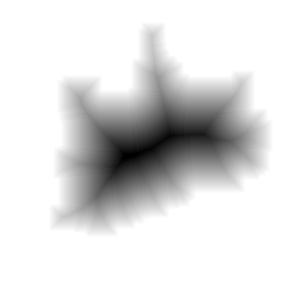
\includegraphics[width=4.5cm]{../C6/EDMFracb}}}
	\\
	\captionsetup[subfloat]{position=top}
	\subfloat[]{\label{fig:EDMFracPlot}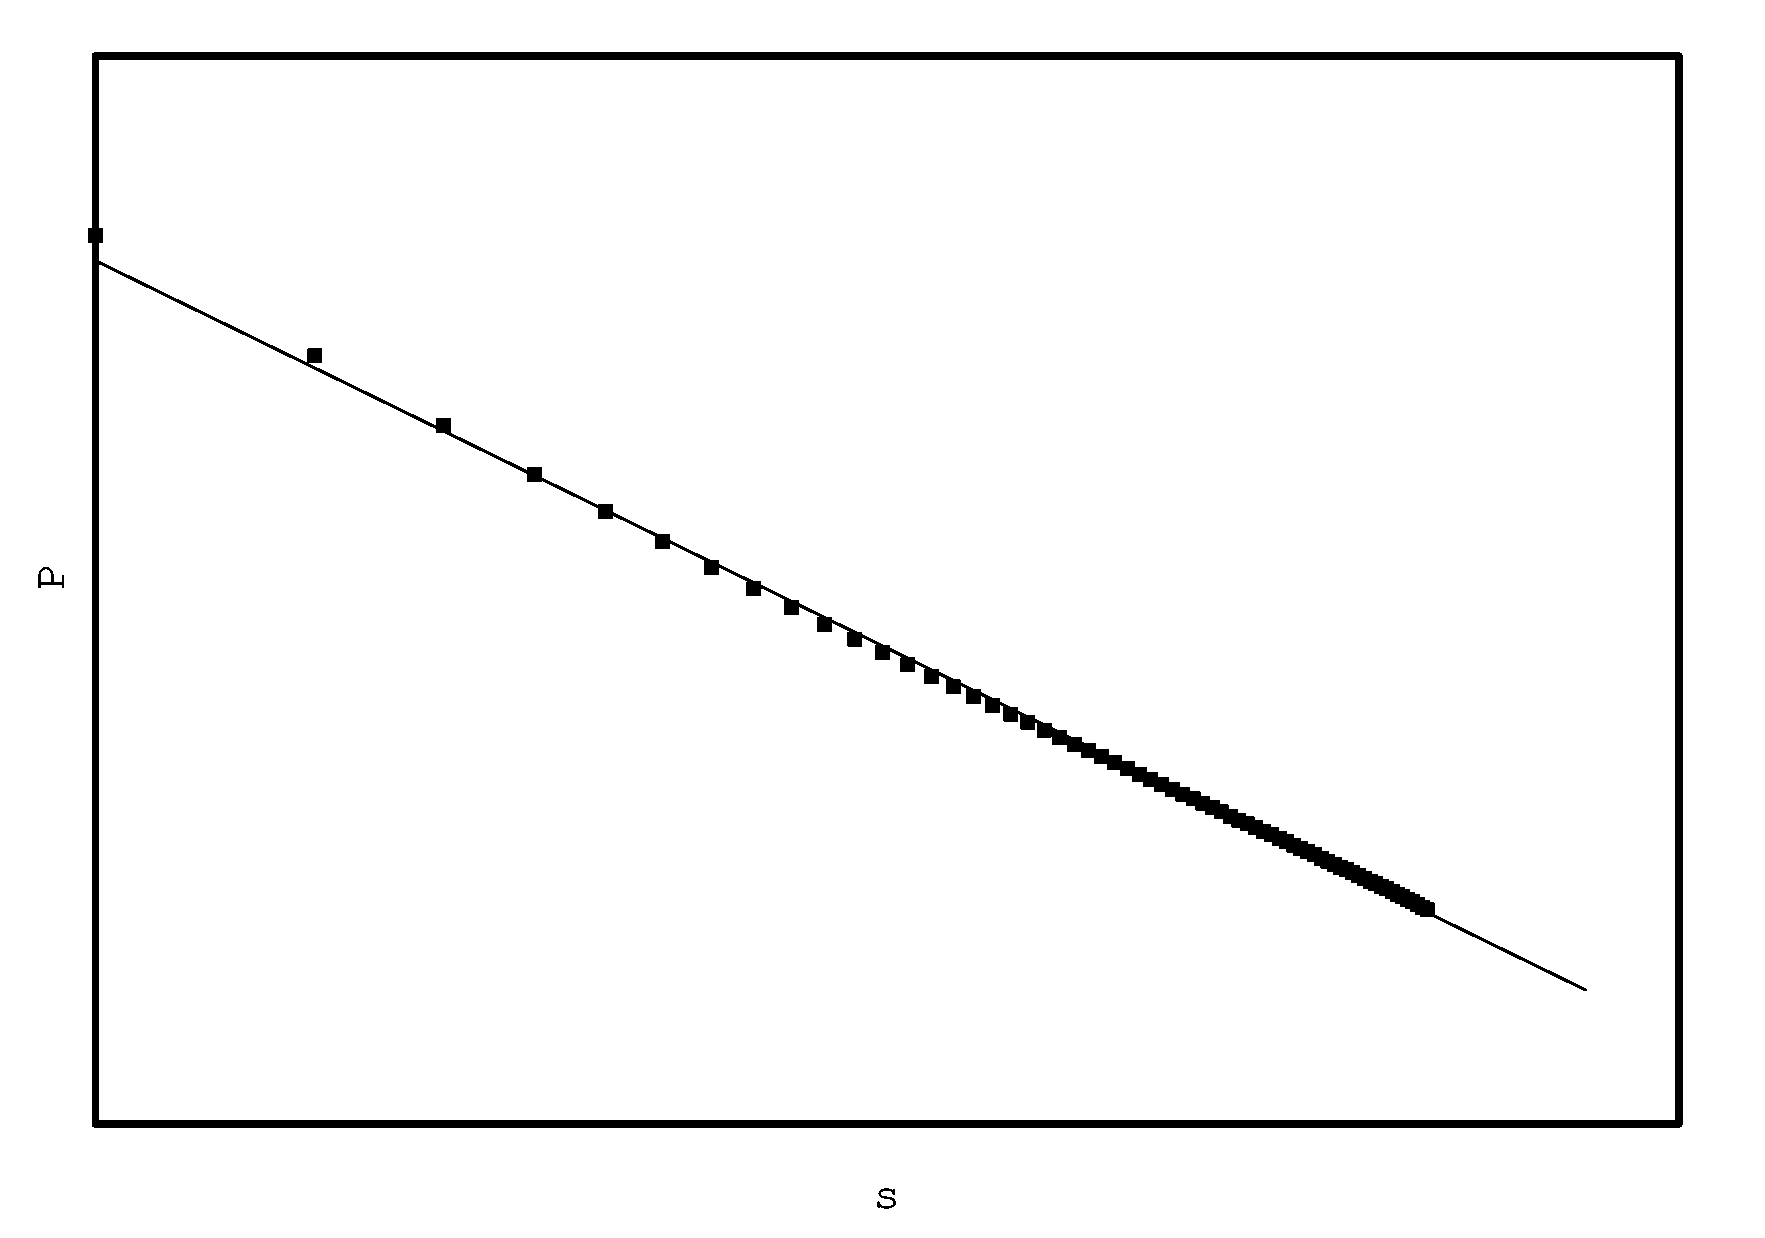
\includegraphics[width=10.5cm]{../C6/EDMFracPlot}}
	\caption{Enumeration of the fractal dimension based on the Euclidean distance map (EDM). (a) Binary representation of object to be analysed. (b) EDM of object in \lq a', in which grey values are inversely proportional to the distance from the nearest background (white) pixel. (c) The fractal dimension may be taken as the slope of a $\log P(d) - \log d$ plot (from Equation~\ref{eq:P(d)}).}
	\label{fig:EDMFrac}
\end{figure}

The \lq box-counting' method has been by far the most common in the analysis of filamentous microbes \cite{obert1990}. This approach entails covering the mycelium with a grid of side length $\epsilon$ and counting the number of boxes, $N(\epsilon)$, that are intersected by the mycelium. If the mycelium is a true fractal, then a relationship of the following form should be found:

\begin{equation} \label{eq:NeD}
	N(\epsilon)=c \epsilon^{-D}
\end{equation}

\noindent where $c$ is a proportionality constant. The fractal nature of mycelia has been studied at two distinct levels using the measures of the surface fractal dimension ($D_{BS}$), effectively allowing discrimination between systems which are fractal only at their boundaries, and the mass fractal dimension ($D_{BM}$) \cite{obert1990,papagianni2006b}. However, it has been suggested that the fractal dimension is often not sufficient for morphological characterisation, as microorganisms can sometimes appear to have different branching patterns, despite having similar values for fractal dimension \cite{boddy2008}.

\subsection{Aim of the work in this chapter}

While numerous studies have been conducted in which fractal analysis is utilised to quantify  morphology, few have attempted to link fractal dimension with conventional morphological parameters. Fractal analysis is of significant potential value in the study of filamentous microorganisms, particularly as it lends itself to the assessment of all gross morphological forms that may be encountered. However, there is a need to develop further the relationship between the fractal dimension within a population of mycelia and the branching behaviour within that population. The aim of this chapter was to investigate an alternative approach to fractal analysis, based on a survey of the mycelial boundary, and attempt to correlate directly the hyphal growth unit ($\hgu$) to the fractal dimension. In order to provide a greater range of $\hgu$ values, \emph{Penicillium chrysogenum} was included in this investigation, as it has been reported to exhibit a more densely branched mycelium with respect to the strain of \emph{A. oryzae} characterised in Chapter~\ref{ch:KinSolidSub} \cite{mcintyre1998,elsabbagh2006}.